% SUBSEÇÃO 1: FUNDAMENDAÇÃO CONCEITO B----------------------------------------------------------------------------
\section{Chatbots}
\label{sec:chatbots}

Tal qual proposto por \citeonline{wezel2020m}, um \textit{chatbot} -- uma contração para o termo \textbf{robo de conversação} (do inglês, \textit{chatting robot}) \cite{lokman2018modern}, é ``uma aplicação baseada em diálogo, projetada para demonstrar comportamento semelhante àquele observado no ser humano''\footnote{``\textit{(...) a dialogue-based program designed to show humanlike behavior (...)}''} \cite[tradução nossa]{wezel2020m} para atender a uma finalidade específica e bem definida.

Pode-se traçar um paralelo entre o surgimento das primeiras aplicações visando esta finalidade -- em meados da década de 1960, com o desenvolvimento da aplicação ELIZA, desenvolvida pelo MIT -- e a evolução dos estudos relacionados à disciplina de NLP \cite{lokman2018modern,allen1988natural}. Todavia, embora tenha permeado o campo computacional desde o seu surgimento, nota-se que o tema ganhou maior relevância recentemente. \citeonline{lokman2018modern} pontuam que tal eminência deve-se, principalmente, ao fato de os dispositivos celulares terem sofrido uma alteração em seu modo de operação: hoje, a troca de mensagens curtas de texto, que representa uma comunicação mais ágil e enxuta, tem-se mostrado o principal uso dos aparelhos, em detrimento à operação por voz, a qual caracteriza um meio de comunicação longo; outro fator que justificaria o recente enfoque ao tópico seria a ``corrida''  disputada pelas grandes corporações na busca de soluções no segmento de assistentes pessoais virtuais (Amazon Alexa, Google Assistant and Apple Siri) \cite{lokman2018modern}.

\subsection{Classificando \textit{chatbots}}
Intentando uma expansão do conceito anteriormente apresentado, pode-se seguir a linha proposta por \citeonline{mctear2020conversational}, o qual pontua que tais sistemas são desenvolvidos para suportar interações com humanos estabelecidas de forma escrita, por fala ou mesmo por ambas as interfaces citadas; tais interações podem ser classificadas em \textbf{diálogos orientados à tarefas}, no qual o ser humano e o sistema estabelecem uma comunicação visando a completude de uma atividade qualquer, e em \textbf{diálogos não orientados a tarefas}, no qual a interação ocorre sem qualquer finalidade pré estabelecida, sendo o objetivo do sistema proporcionar àqueles que com ele interagem uma experiência póxima à comunicação rotineira obervada entre seres humanos \cite{wezel2020m}, a qual é possibilitada graças à existência e à aplicação das técnicas de Processamento de Linguagem Natural \cite{lokman2018modern}. Ainda em relação à classificação dos \textit{chatbots}, \citeonline{lokman2018modern} propoem uma segmentação mais especializada, conforme elencado nos tópicos adiante, categorizando-os de acordo características observadas a partir de seu projeto; um resumo gráfico, agrupando ambos os sistemas de classificação podem ser verificados na Figura\ref{fig:M2}

\begin{enumerate}
    \item \textbf{Domínio de conhecimento}: \textit{chatbots} podem ser categorizados como de \textbf{domínio aberto} -- quando o sistema intenta cobrir uma gama esparsa de tópicos recentes, de assuntos relacionados a entretenimento e afins, estabelecendo um diálogo sem escopo definido com o humano que o opera (cuja implementação demonstra-se mais complexa e com resultados menos confiáveis em relação à sua contraparte), ou de \textbf{domínio fechado} -- quando projetado para operar sobre uma área de domínio específico, tal qual serviço ao cliente ou psicologia (de mais fácil construção e com resultados consideravelmente robustos) \cite{lokman2018modern}..
    % \textit{Chatbots} de domínio de conhecimento aberto consomem uma grande variedade de \textit{datasets}, além de executarem um trabalho de \textit{web scrapping} em resultados obtidos a partir de mecanismos de busca (tal qual Google, Bing e DuckDuckGo) ou repositórios de conhecimento (como a Wikipedia), serviços de redes sociais (como Twitter ou Reddit), para construir sua base de conhecimento; em contrapartida \textit{chatbots} de domínio de conhecimento demandam uma base oriunda de um trabalho mais especializado. fechado tendem a ser de mais fácil implementação, angariando bons resultados, enquanto que aqueles que operam em cima de um domínio aberto continuam a apresentar desafios de contrução, produzindo uma quantidade considerável de resultados falso positivos \cite{lokman2018modern}.
    
    \item \textbf{Geração de Respostas}: há dois métodos principais, sob os quais todas as demais estratégias podem ser agrupadas, em relação a como os \textit{chatbots} produzem as respostas fornecidas ao usuários: \textbf{recuperação} e \textbf{geração}; o primeiro método é um processo que seleciona a melhor saída a partir de uma lista préviamente selecionada, enquanto o segundo baseia seu retorno a partir da sequência de entrada fornecida pelo operador da aplicação, a qual é submetida a classificadores treinados. Uma importante observação é que aplicações baseadas em diálogo podem aplicar ambas as técnicas em sua construção, operando em um modelo híbrido \cite{lokman2018modern}.
    \item \textbf{Processamento de Texto}: esta caracteriza implica em como o \textit{chatbot} processa o texto, o que habilita de fato o seu funcionamento; há um certo consenso aqui sobre o uso de vetores de incorporação (uma tradução livre para o termo original, em inglês, \textit{word embedding}), que buscam representar relacionamento semânticos entre palavras dentro de um determinado vocabulário na forma de números reais em um espaço vetorial, o que possibilita que operações estatísticas -- e mesmo aritméticas -- sejam aplicadas sem grandes dificuldades. Todavia, há ainda uma corrente que emprega palavras -- ou mesmo caracteres -- do alfabeto latino como informação de entrada e saída em seu processamento.
    \item \textbf{Modelos de Aprendizado de Máquina}: deve-se observar que nem todos os chatbots empregam modelos de aprendizado de máquina em sua implementação -- conforme apontado anteriormenrte, as implementações se dividem, em relação ao modo como processam o texto para alimentar a aplicação, entre as que apenas processam a entrada e a saída baseadas em palvras ou caracteres e as recorrem ao uso de \textit{word embeddings}. Invariavelmente, as soluções que fazem uso da segunda abordagem, possuem duas formas de produzir os vetores mencionados: por contagem de coocorrências de palavras em um contexto específico, o qual não utiliza aprendizado de máquina, e pela predição dos termos em si, utilizando os modelos mencionados; embora pareça improvável, o método por predição tem se demonstrado superior método por contagem real, habilitando-o como principal estratégia de implementação de chatbots.
\end{enumerate}


\begin{figure}[htb!]
    \centering    
    \caption{Classificação das aplicações de chatbots de acordo com caracteríscas de escopo}
    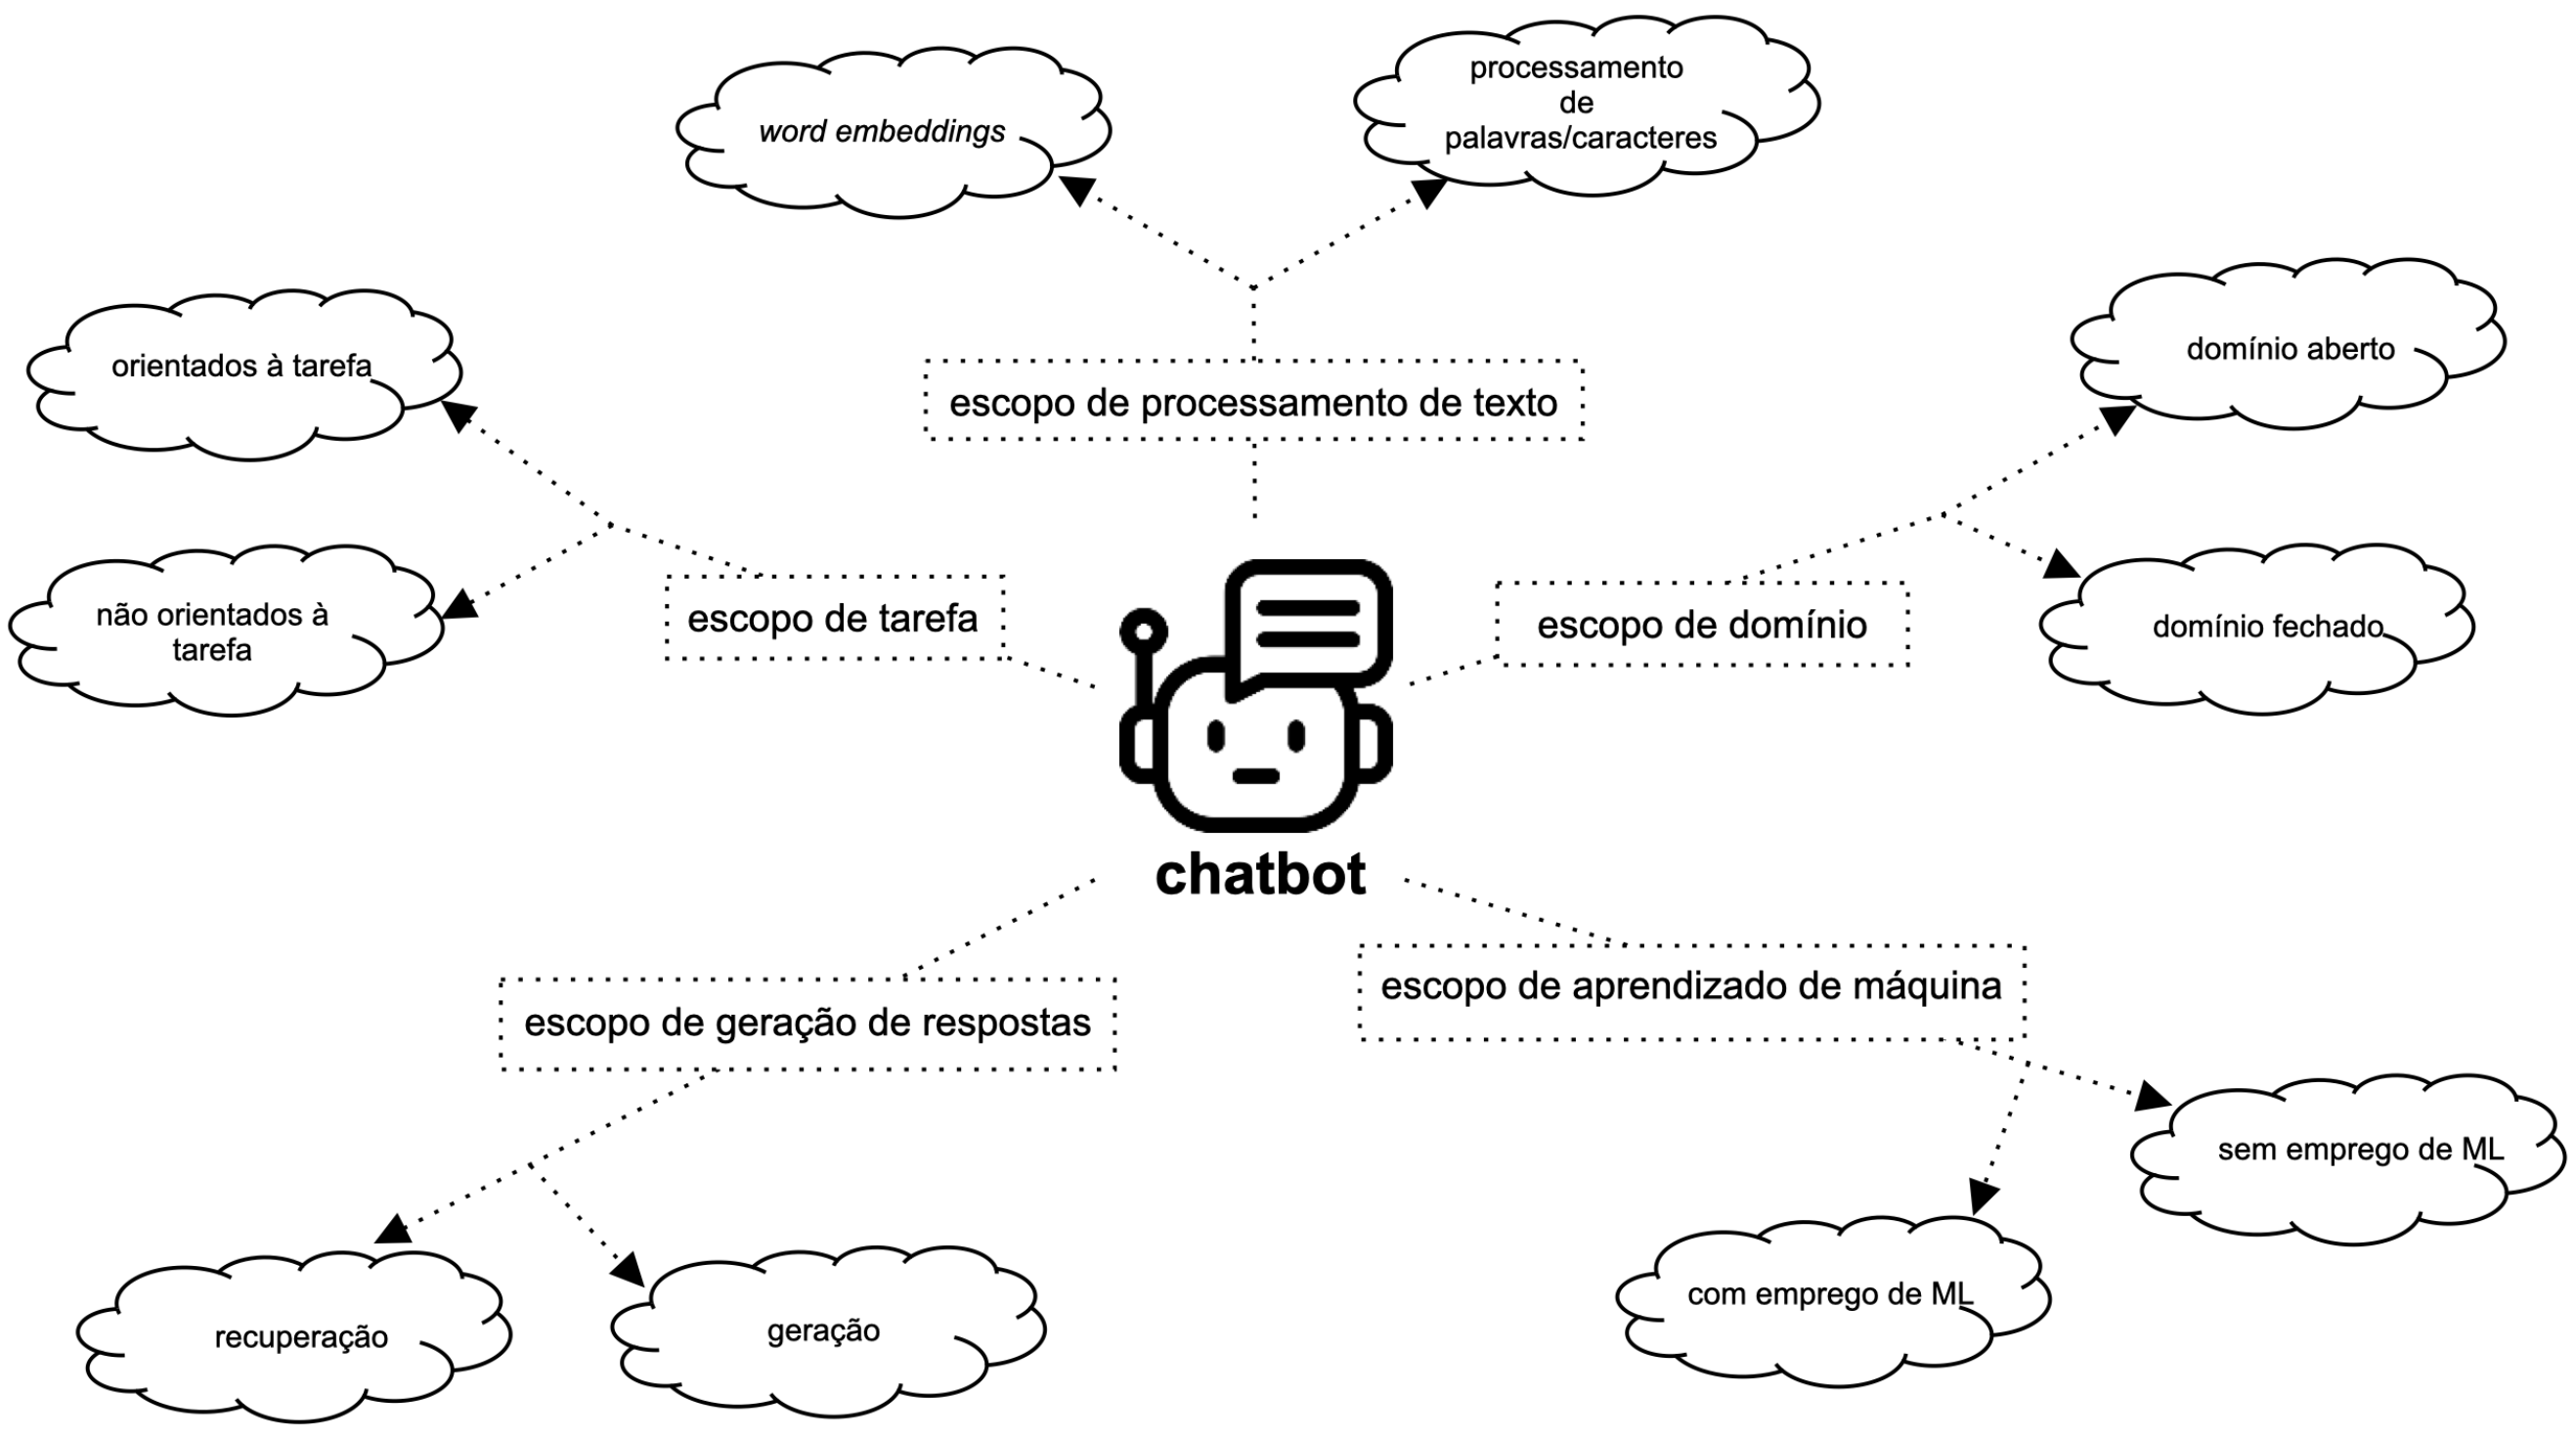
\includegraphics[width=1\linewidth]{estrutura/img/classificacao_chatbots.png}
    \fonte{O autor\footnotemark}
    \label{fig:M2}
\end{figure}

\footnotetext{Construída baseando-se no material proposto por \citeonline{lokman2018modern} e \citeonline{allen1988natural}}